%!TEX root = ../main.tex

\chapter{Einleitung} % (fold)
% \addcontentsline{toc}{chapter}{Einleitung}
\label{cha:einleitung}

Lorem ipsum dolor sit amet, consectetur adipisicing elit, sed do eiusmod
tempor incididunt ut labore et dolore magna aliqua. Ut enim ad minim veniam,
quis nostrud exercitation ullamco laboris nisi ut aliquip ex ea commodo
consequat. Duis aute irure dolor in reprehenderit in voluptate velit esse
cillum dolore eu fugiat nulla pariatur. Excepteur sint occaecat cupidatat non
proident, sunt in culpa qui officia deserunt mollit anim id est laborum.

Lorem ipsum dolor sit amet, consectetur adipisicing elit, sed do eiusmod
tempor incididunt ut labore et dolore magna aliqua. Ut enim ad minim veniam,
quis nostrud exercitation ullamco laboris nisi ut aliquip ex ea commodo
consequat. Duis aute irure dolor in reprehenderit in voluptate velit esse
cillum dolore eu fugiat nulla pariatur. Excepteur sint occaecat cupidatat non
proident, sunt in culpa qui officia deserunt mollit anim id est laborum.

Lorem ipsum dolor sit amet, consectetur adipisicing elit, sed do eiusmod
tempor incididunt ut labore et dolore magna aliqua. Ut enim ad minim veniam,
quis nostrud exercitation ullamco laboris nisi ut aliquip ex ea commodo
consequat. Duis aute irure dolor in reprehenderit in voluptate velit esse
cillum dolore eu fugiat nulla pariatur. Excepteur sint occaecat cupidatat non
proident, sunt in culpa qui officia deserunt mollit anim id est laborum.

\section{Motivation} % (fold)
\label{sec:motivation}

Ein Polymer, oder auch Makromolekül, ist ein Molekül, welches sich aus vielen kleineren, sich wiederholenden Molekülen, sogenannten Monomeren, zusammensetzt.
Besteht ein Polymer aus nur einer Monomer-Art, dann spricht man von einem Homopolymer, sonst von einem Heteropolymer oder auch Copolymer.
Typischerweise besteht ein Polymer aus einer langen Kette von aneinanderhängenden Monomeren, es existieren aber auch weitere Konfigurationen, zum Beispiel stern- oder ringförmige Anordnungen.

Copolymere lassen sich anhand der Anordnung der Monomere weiter klassifizieren.
Bilden die verschiedenen Monomer-Gattungen homogene, zusammenhängede Gruppen, welche wiederum durch aneinanderreihen das Copolymer bilden, dann nennen wir dies ein Blockcopolymer.

Es existieren unüberschaubar viele solcher Konfigurationen von Polymeren, und insbesondere Blockcopolymeren, vergleiche \autoref{fig:konfig}, weswegen man häufig auf das Studium vergleichsweise simpler Anordnungen zurückgreift.
Als besonders beliebt hat sich der Fall des kettenförmigen Blockcopolymers mit zwei Monomer-Typen, der Einfachheit halber A und B genannt, herausgestellt.
Diese Konfiguration wird auch als AB-Diblockcopolymer bezeichnet.

\begin{figure}[tb]
    \centering
    % \includegraphics[]{}
    \missingfigure{}
    \caption{%
        Skizzenhafte Darstellung eines Homopolymers, eines sogenannten statistischen AB-Copolymers, bei dem die beiden Monomer-Arten zufällig verteilt sind, und eines AB-Diblockcopolymers.
    }
    \label{fig:konfig}
\end{figure}

Von großem Interesse ist das Verhalten von Gemischen verschiedener Polymer-Arten.
So neigen viele Paare von Homopolymeren zu makroskopischer Phasenseparation, wie man es zum Beispiel von Öl und Essig kennt.
Eine ähnliche Tendenz findet man auch bei Blockcopolymeren, hierbei kann aufgrund der Verbindung der verschiedenen Monomer-Blöcke aber keine makroskopische Phasenseparation auftreten.
Stattdessen kommt es zu einer periodischen, mikroskopischen Separation.
\autoref{fig:anordnungen} zeigt einige mögliche Anordnungen, die bei Diblockcopolymeren tatsächlich experimentell beobachtet wurden.

\begin{figure}[tb]
    \centering
    \begin{subfigure}[b]{0.18\textwidth}
        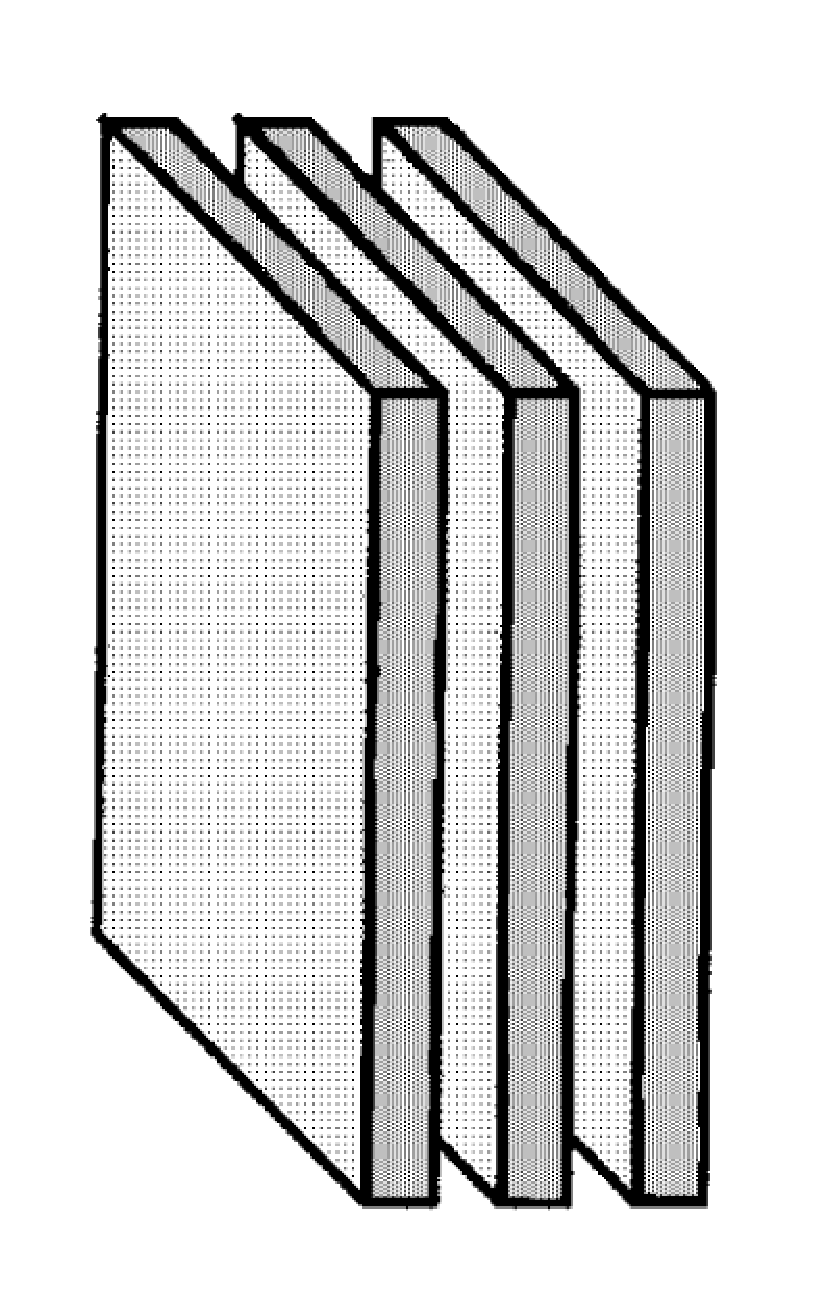
\includegraphics[width=\textwidth]{figures/einleitung/fig1}
    \end{subfigure}
    \begin{subfigure}[b]{0.18\textwidth}
        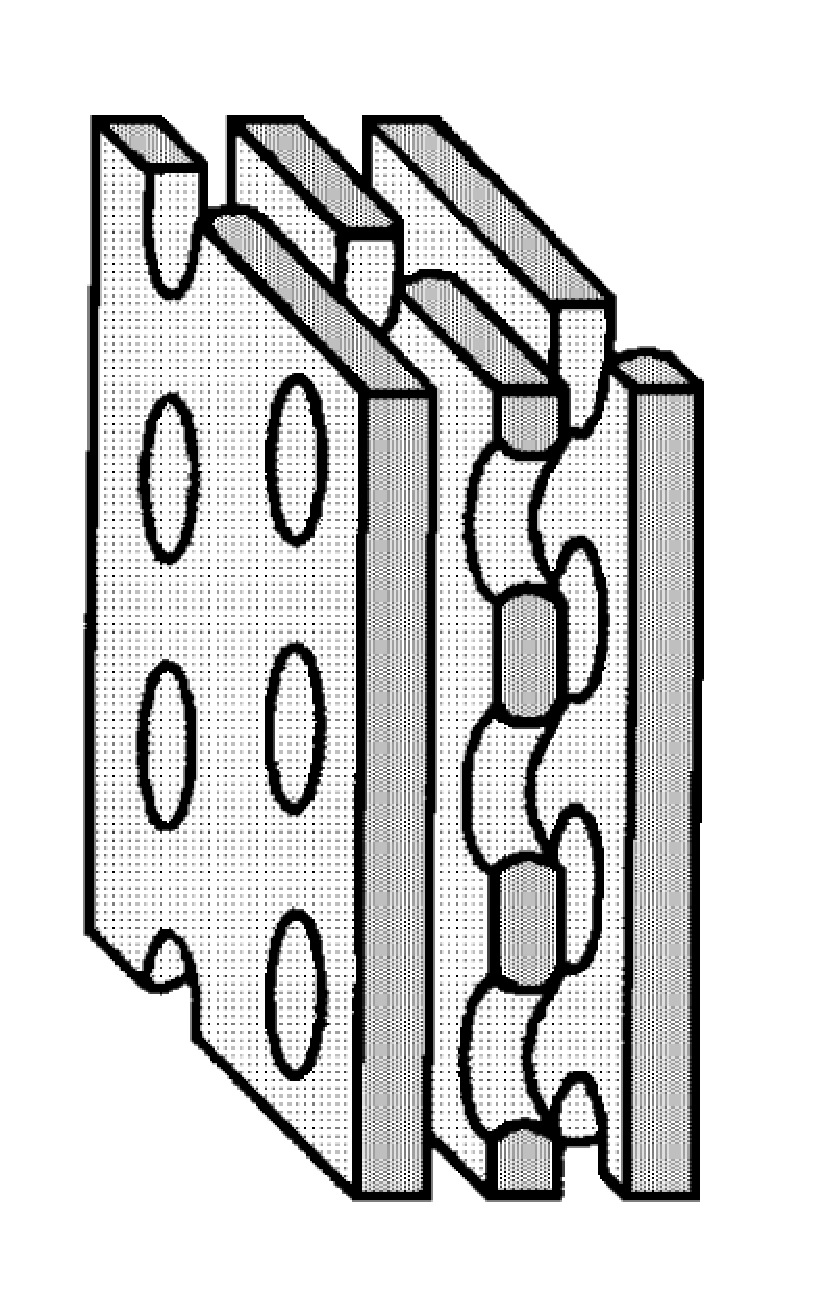
\includegraphics[width=\textwidth]{figures/einleitung/fig2}
    \end{subfigure}
    \begin{subfigure}[b]{0.18\textwidth}
        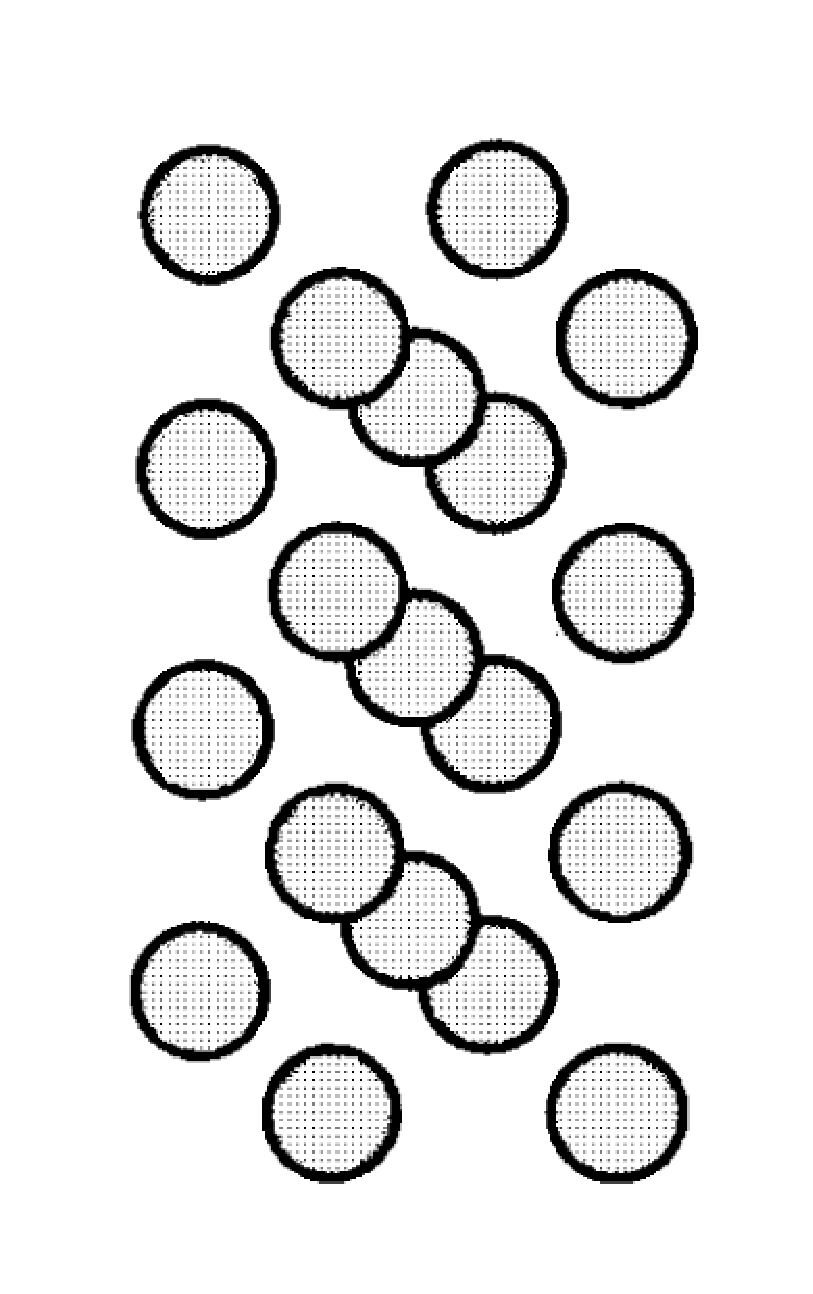
\includegraphics[width=\textwidth]{figures/einleitung/fig3}
    \end{subfigure}
    \begin{subfigure}[b]{0.18\textwidth}
        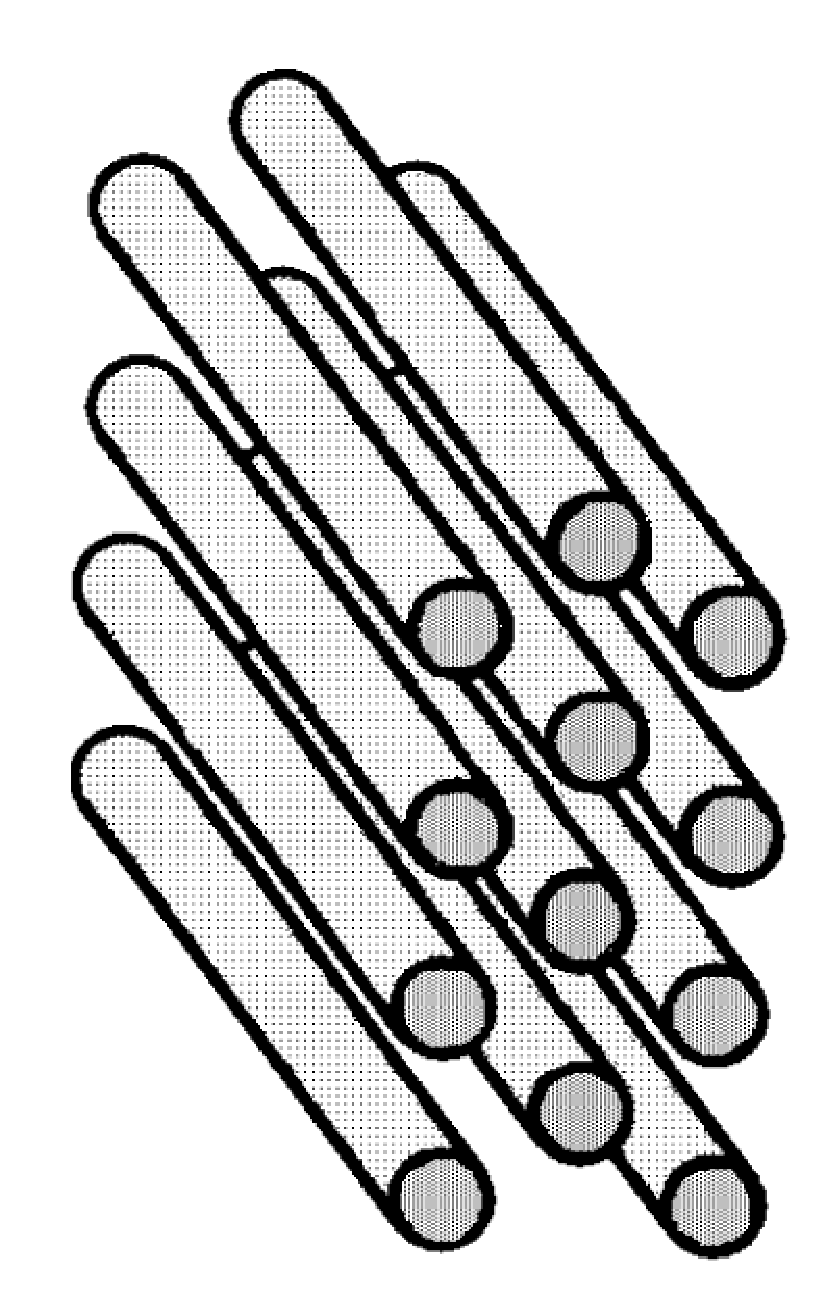
\includegraphics[width=\textwidth]{figures/einleitung/fig4}
    \end{subfigure}
    \begin{subfigure}[b]{0.18\textwidth}
        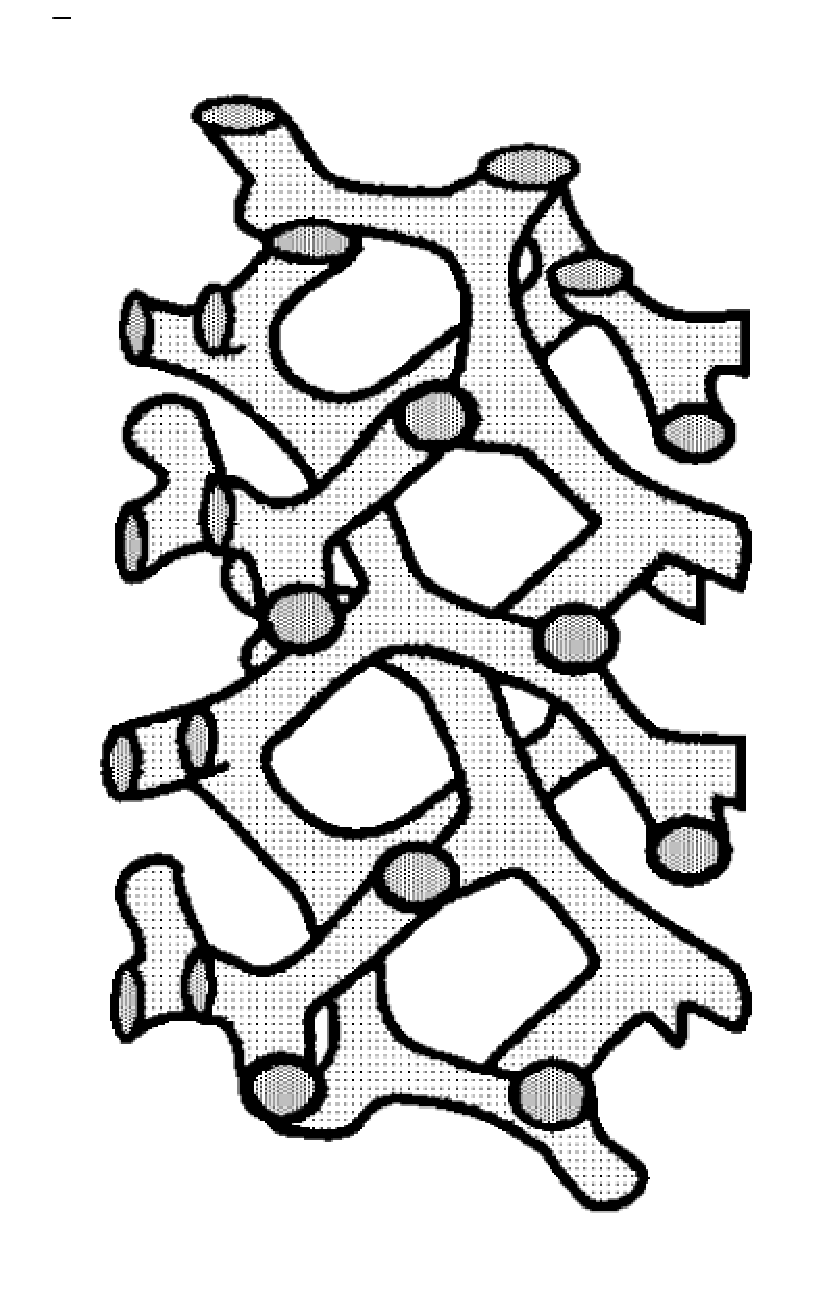
\includegraphics[width=\textwidth]{figures/einleitung/fig5}
    \end{subfigure}
    \caption{%
        Verschiedene Phasen bei Diblockcopolymeren, welche experimentell beobachtet wurden, wobei hierbei nur eine der beiden Monomer-Gattungen dargestellt wird.
        Diese heißen von links nach rechts: Lamellar, Perforiert-Lamellar, Sphärisch, Zylindrisch, Gyroid.
        Diese Abbildung wurde \cite[Figure 1.18]{Matsen:2006ud} entnommen.
    }
    \label{fig:anordnungen}
\end{figure}

Da die experimentelle Bestimmung ohne Vorwissen über die möglichen, stabilen Anordnungen nur wenig erfolgversprechend ist, wird eine fundierte Theorie benötigt, auf Basis derer theoretische Vorhersagen getroffen werden können, die vorzugsweise wiederum experimentell belegt werden können.
Da außerdem Diblockcopolymere einen relativ simplen Fall eines Copolymers darstellen, wurde sowohl in die experimentelle als auch theoretische Untersuchung dieser bereits vergleichsweise viel Arbeit investiert.

Als besonders nützliche und dennoch relativ einfache Theorie hat sich das auf der sogenannten selbstkonsistenten Feldtheorie, im Weiteren wird der englische Ausdruck \emph{self-consistent-field-theory}, kurz SCFT, verwendet, basierende Modell herausgestellt.

% subsection polymere (end)

Es folgt eine sehr einfach gehaltene Einführung in die SCFT für Diblock-Copolymere.

Because SCFT has become a standard theoretical method for studying block copoly- mer phase behavior, only a brief summary is given here. The theory provides a statistical description of the spatial distribution of interacting chain segments. It has two basic ingredients: chain configurations are described as random walks; monomer- monomer interactions are replaced by interactions between monomers and self-consis- tently determined molecular fields.

Die selbstkonsistente Feldtheorie, im Weiteren wird der englische Ausdruck \emph{self-consistent-field-theory}, kurz SCFT, verwendet, ist ein weit verbreitetes theoretisches Modell der Physik um das Verhalten von Teilchen unter Einwirkung von Kräften, die durch Wechselwirkung mit anderen Teilchen auftreten, zu studieren.
Mit Hilfe dieses Modells lässt sich die statistische räumliche Verteilung eines Teilchens bestimmen.
Hierbei wird zur Vereinfachung des Modells das eigentlich vorliegende Mehrkörperproblem durch mitteln der Wechselwirkungen auf ein Einkörperproblem reduziert.


\section{Bisherige Numerische Methoden} % (fold)
\label{sec:bisherige_numerische_methoden}

Lorem ipsum dolor sit amet, consectetur adipisicing elit, sed do eiusmod
tempor incididunt ut labore et dolore magna aliqua. Ut enim ad minim veniam,
quis nostrud exercitation ullamco laboris nisi ut aliquip ex ea commodo
consequat. Duis aute irure dolor in reprehenderit in voluptate velit esse
cillum dolore eu fugiat nulla pariatur. Excepteur sint occaecat cupidatat non
proident, sunt in culpa qui officia deserunt mollit anim id est laborum.

Lorem ipsum dolor sit amet, consectetur adipisicing elit, sed do eiusmod
tempor incididunt ut labore et dolore magna aliqua. Ut enim ad minim veniam,
quis nostrud exercitation ullamco laboris nisi ut aliquip ex ea commodo
consequat. Duis aute irure dolor in reprehenderit in voluptate velit esse
cillum dolore eu fugiat nulla pariatur. Excepteur sint occaecat cupidatat non
proident, sunt in culpa qui officia deserunt mollit anim id est laborum.

Lorem ipsum dolor sit amet, consectetur adipisicing elit, sed do eiusmod
tempor incididunt ut labore et dolore magna aliqua. Ut enim ad minim veniam,
quis nostrud exercitation ullamco laboris nisi ut aliquip ex ea commodo
consequat. Duis aute irure dolor in reprehenderit in voluptate velit esse
cillum dolore eu fugiat nulla pariatur. Excepteur sint occaecat cupidatat non
proident, sunt in culpa qui officia deserunt mollit anim id est laborum.


\section{Aufbau und Ziele dieser Arbeit} % (fold)
\label{sec:aufbau_und_ziele_dieser_arbeit}

Lorem ipsum dolor sit amet, consectetur adipisicing elit, sed do eiusmod
tempor incididunt ut labore et dolore magna aliqua. Ut enim ad minim veniam,
quis nostrud exercitation ullamco laboris nisi ut aliquip ex ea commodo
consequat. Duis aute irure dolor in reprehenderit in voluptate velit esse
cillum dolore eu fugiat nulla pariatur. Excepteur sint occaecat cupidatat non
proident, sunt in culpa qui officia deserunt mollit anim id est laborum.

Lorem ipsum dolor sit amet, consectetur adipisicing elit, sed do eiusmod
tempor incididunt ut labore et dolore magna aliqua. Ut enim ad minim veniam,
quis nostrud exercitation ullamco laboris nisi ut aliquip ex ea commodo
consequat. Duis aute irure dolor in reprehenderit in voluptate velit esse
cillum dolore eu fugiat nulla pariatur. Excepteur sint occaecat cupidatat non
proident, sunt in culpa qui officia deserunt mollit anim id est laborum.

Lorem ipsum dolor sit amet, consectetur adipisicing elit, sed do eiusmod
tempor incididunt ut labore et dolore magna aliqua. Ut enim ad minim veniam,
quis nostrud exercitation ullamco laboris nisi ut aliquip ex ea commodo
consequat. Duis aute irure dolor in reprehenderit in voluptate velit esse
cillum dolore eu fugiat nulla pariatur. Excepteur sint occaecat cupidatat non
proident, sunt in culpa qui officia deserunt mollit anim id est laborum.

% chapter einleitung (end)
